%%%%%%%%%%%%%%%%%%%%%%%%%%%%%%%%%%%%%%%%%
% Beamer Presentation
% LaTeX Template
% Version 1.0 (10/11/12)
%
% This template has been downloaded from:
% http://www.LaTeXTemplates.com
%
% License:
% CC BY-NC-SA 3.0 (http://creativecommons.org/licenses/by-nc-sa/3.0/)
%
%%%%%%%%%%%%%%%%%%%%%%%%%%%%%%%%%%%%%%%%%

%----------------------------------------------------------------------------------------
%	PACKAGES AND THEMES
%----------------------------------------------------------------------------------------

\documentclass{beamer}
\usepackage[spanish]{babel}
\usepackage[utf8]{inputenc}
\mode<presentation> {

% The Beamer class comes with a number of default slide themes
% which change the colors and layouts of slides. Below this is a list
% of all the themes, uncomment each in turn to see what they look like.

%\usetheme{default}
%\usetheme{AnnArbor}
%\usetheme{Antibes}
%\usetheme{Bergen}
%\usetheme{Berkeley}
%\usetheme{Berlin}
%\usetheme{Boadilla}
%\usetheme{CambridgeUS}
%\usetheme{Copenhagen}
%\usetheme{Darmstadt}
%\usetheme{Dresden}
%\usetheme{Frankfurt}
%\usetheme{Goettingen}
%\usetheme{Hannover}
%\usetheme{Ilmenau}
%\usetheme{JuanLesPins}
%\usetheme{Luebeck}
%\usetheme{Madrid}
%\usetheme{Malmoe}
%\usetheme{Marburg}
%\usetheme{Montpellier}
\usetheme{PaloAlto}
%\usetheme{Pittsburgh}
%\usetheme{Rochester}
%\usetheme{Singapore}
%\usetheme{Szeged}
%\usetheme{Warsaw}

% As well as themes, the Beamer class has a number of color themes
% for any slide theme. Uncomment each of these in turn to see how it
% changes the colors of your current slide theme.

%\usecolortheme{albatross}
%\usecolortheme{beaver}
%\usecolortheme{beetle}
%\usecolortheme{crane}
%\usecolortheme{dolphin}
%\usecolortheme{dove}
%\usecolortheme{fly}
%\usecolortheme{lily}
%\usecolortheme{orchid}
%\usecolortheme{rose}
%\usecolortheme{seagull}
%\usecolortheme{seahorse}
%\usecolortheme{whale}
%\usecolortheme{wolverine}

%\setbeamertemplate{footline} % To remove the footer line in all slides uncomment this line
%\setbeamertemplate{footline}[page number] % To replace the footer line in all slides with a simple slide count uncomment this line

%\setbeamertemplate{navigation symbols}{} % To remove the navigation symbols from the bottom of all slides uncomment this line
}

\usepackage{graphicx} % Allows including images
\usepackage{booktabs} % Allows the use of \toprule, \midrule and \bottomrule in tables

%----------------------------------------------------------------------------------------
%	TITLE PAGE
%----------------------------------------------------------------------------------------

\title[Practica 1]{Practica 1: Eficiencia} % The short title appears at the bottom of every slide, the full title is only on the title page

\author{Algoritmica} % Your name
\institute[UGR] % Your institution as it will appear on the bottom of every slide, may be shorthand to save space
{
Universidad de Granada \\ % Your institution for the title page
\medskip

}
\date{\today} % Date, can be changed to a custom date

\begin{document}

\begin{frame}
\titlepage % Print the title page as the first slide
\end{frame}

\begin{frame}
\frametitle{Indice} % Table of contents slide, comment this block out to remove it
\tableofcontents % Throughout your presentation, if you choose to use \section{} and \subsection{} commands, these will automatically be printed on this slide as an overview of your presentation
\end{frame}

%----------------------------------------------------------------------------------------
%	PRESENTATION SLIDES
%----------------------------------------------------------------------------------------

\section{Introducción }
\begin{frame}
	\frametitle{Introducción}
	\begin{itemize}
		\item El objetivo de ésta práctica es analizar eficiencias de forma empírica e híbrida.
		\item Para ello, hemos recogido los diferentes tiempos de los diferentes algoritmos que se ofrecían y los hemos comparado.
		\item En nuestro caso concreto, hemos utilizado la biblioteca de C++ más moderna y precisa destinado a obtener tiempos de reloj: la biblioteca \textbf{chrono}
		\end{itemize}
\end{frame}
\begin{frame}
	\frametitle{Especificaciones de la máquina}
	\begin{itemize}
		
		\item Procesador: Intel Core i5-3337U (2.7GHz x 2)
		\item Memoria RAM: 4GB
	    \item Disco Duro: 500GB 5400 rpm
		\item SO: Manjaro Linux 15.2 Capella 64 bits
	\end{itemize}
	
\end{frame}


%------------------------------------------------
\section{Ordenación} % Sections can be created in order to organize your presentation into discrete blocks, all sections and subsections are automatically printed in the table of contents as an overview of the talk
%------------------------------------------------
\begin{frame}
	\frametitle{Ordenación}
	Según hemos ido hemos estudiado, estos algoritmos que presentamos tienen teóricamente y calculando a partir del código una eficiencia de $O(n^2 )$. Como esto es teórico, vamos a ver si efectivamente (o no) los algoritmos proporcionados se parecen a la gráfica de $n^2$ recogiendo la información de 99 posibilidades distintas en cada algoritmo.
	\begin{figure}
		\centering
		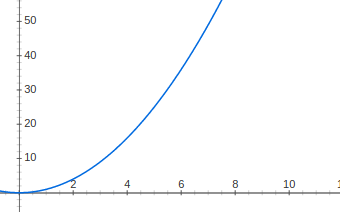
\includegraphics[width=0.7\linewidth]{imagenes/enecuadrado.png}
		\caption{}
		\label{fig:E1}
	\end{figure}

\end{frame}

\subsection{Burbuja}
\begin{frame}
	\frametitle{Burbuja}
	La gráfica empírica obtenida ha sido:
	\begin{figure}
		\centering
		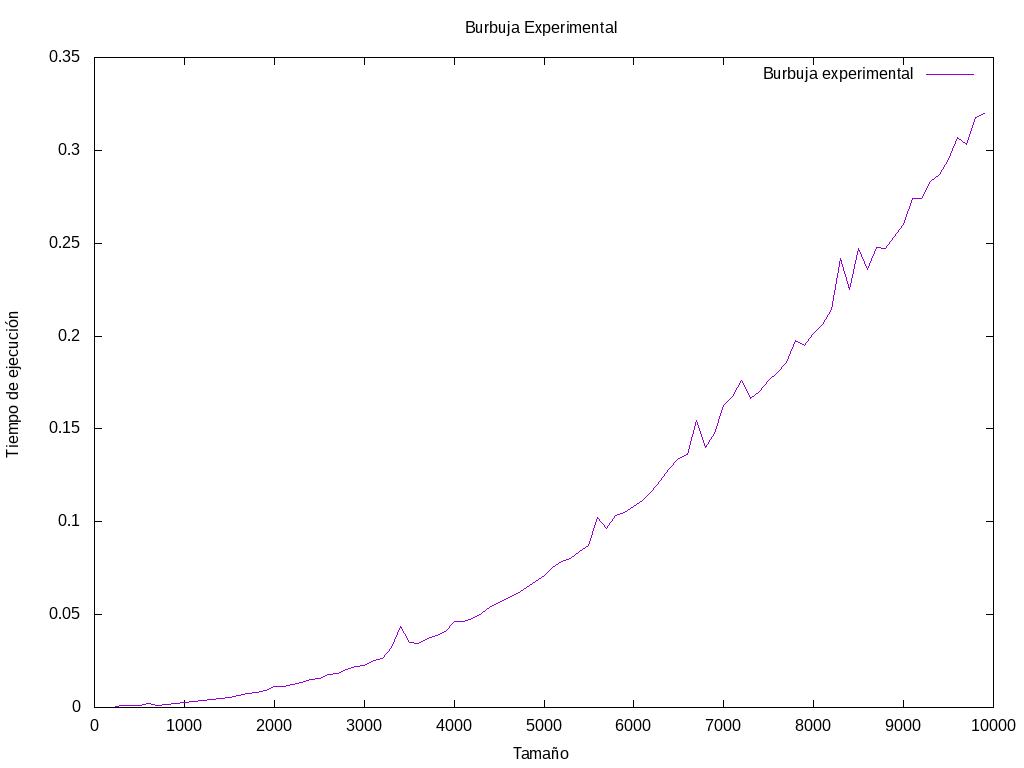
\includegraphics[width=0.7\linewidth]{imagenes/burbuja-experimental.png}
		\caption{}
		\label{fig:E2}
	\end{figure}
	
\end{frame}

\begin{frame}
	\frametitle{Burbuja}
	La gráfica híbrida obtenida ha sido:
	\begin{figure}
		\centering
		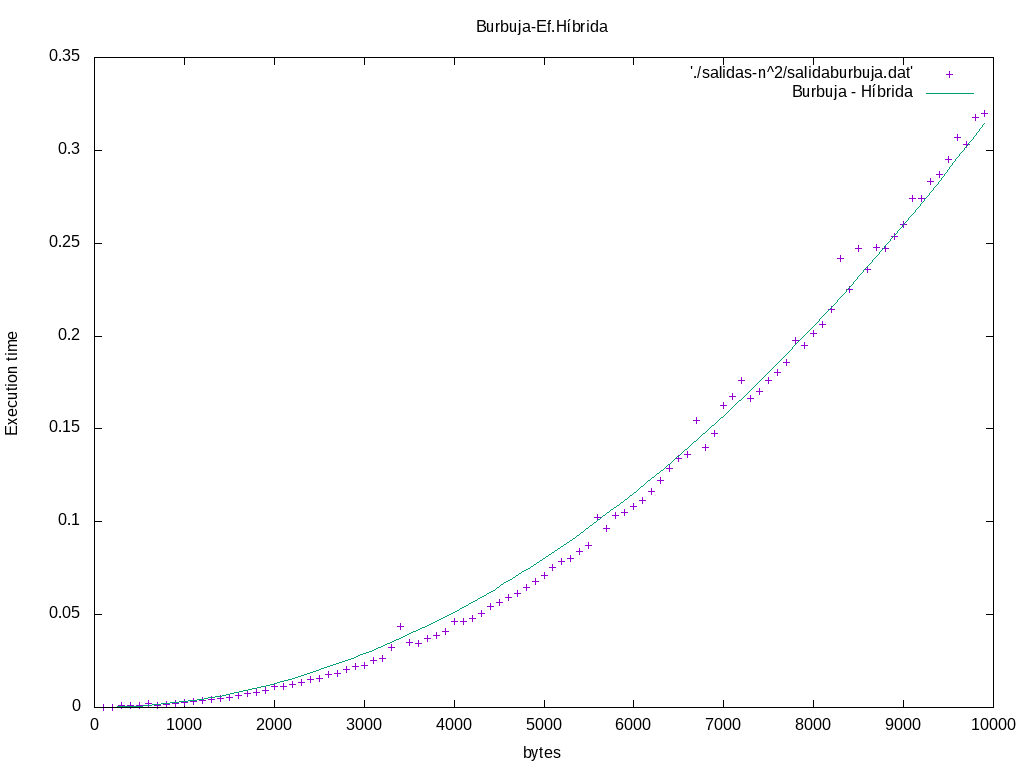
\includegraphics[width=0.7\linewidth]{imagenes/burbuja-hibrida.png}
		\caption{}
		\label{fig:E3}
	\end{figure}	
\end{frame}





\subsection{Selección}
\begin{frame}
	\frametitle{Selección}
	La gráfica empírica obtenida ha sido:
	\begin{figure}
		\centering
		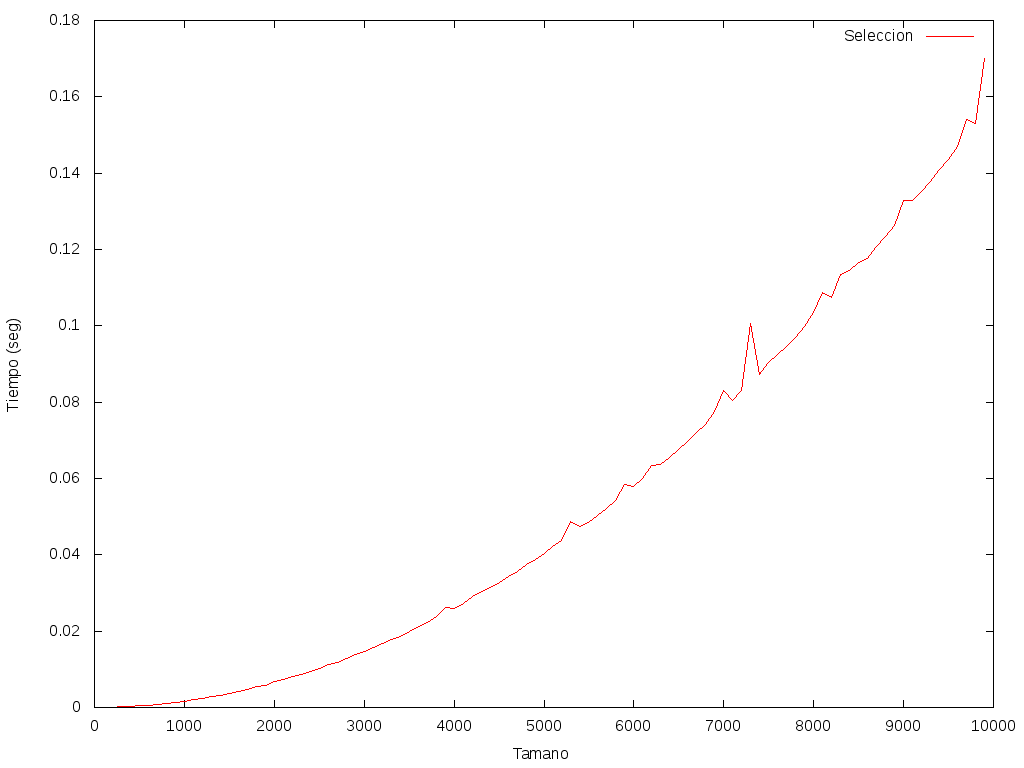
\includegraphics[width=0.7\linewidth]{imagenes/seleccionLines.png}
		\caption{}
		\label{fig:E4}
	\end{figure}
	
\end{frame}

\begin{frame}
	\frametitle{Selección}
	La gráfica híbrida obtenida ha sido:
	\begin{figure}
		\centering
		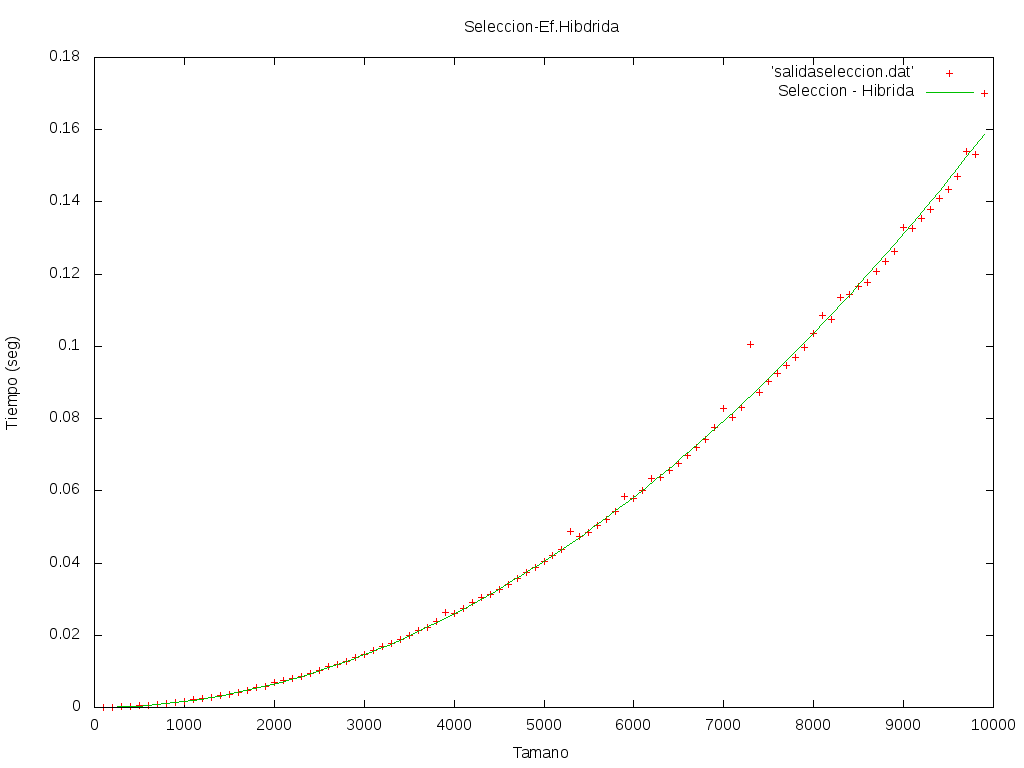
\includegraphics[width=0.7\linewidth]{imagenes/seleccion-hibrida.png}
		\caption{}
		\label{fig:E5}
	\end{figure}
	
\end{frame}
\subsection{Inserción}
\begin{frame}
	\frametitle{Inserción}
	La gráfica empírica obtenida ha sido:
	\begin{figure}
		\centering
		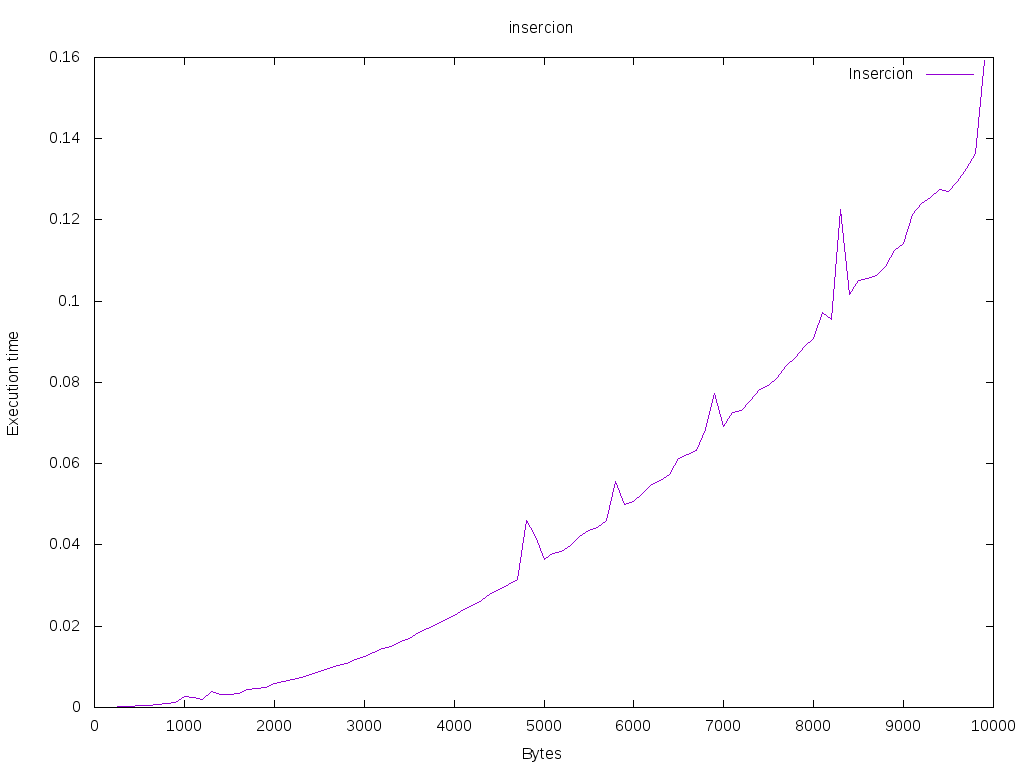
\includegraphics[width=0.7\linewidth]{imagenes/insercion.png}
		\caption{}
		\label{fig:E2}
	\end{figure}
	
\end{frame}

\begin{frame}
	\frametitle{Inserción}
	La gráfica híbrida obtenida ha sido:
	\begin{figure}
		\centering
		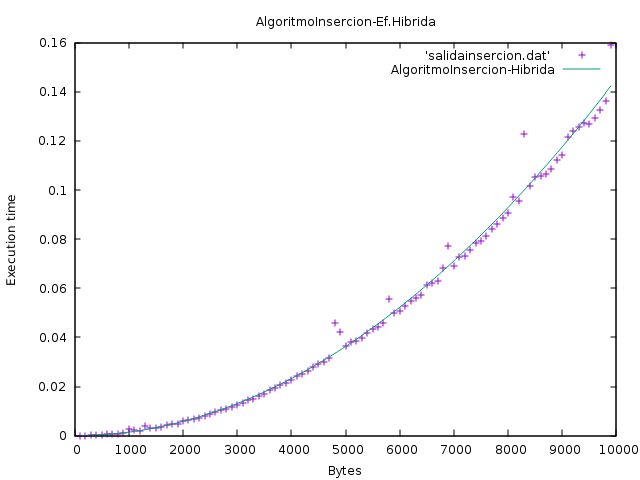
\includegraphics[width=0.7\linewidth]{imagenes/algoritmoInsercion-hibrida}
		\caption{}
		\label{fig:E3}
	\end{figure}
	
\end{frame}


\begin{frame}
	\frametitle{Algoritmos $n^2$}
	Por ultimo, mostramos el porcentaje de error a la hora de obtener las constantes ocultas es muy bajo.\\
	
	\begin{center}
		\begin{tabular}{| l | c | r |}
			\hline
			\textbf{Algoritmo} & \textbf{Constante Oculta} & \textbf{Error} \\ \hline
			Burbuja & a0 = 3.20873e-09 & +/- 1.403e-11 (0.4372\%)\\ \hline
			Selección & a0 = 1.61988e-09 & +/- 4.818e-12 (0.2975\%) \\ \hline
			Inserción & a0 = 1.45151e-09 &  +/- 8.337e-12    (0.5743\%) \\ \hline
		\end{tabular}
	\end{center}

	
	
\end{frame}


\section{Ordenación rápida} % Sections can be created in order to organize your presentation into discrete blocks, all sections and subsections are automatically printed in the table of contents as an overview of the talk
%------------------------------------------------
\begin{frame}
	\frametitle{Ordenación rápida}
	Según hemos ido estudiado, estos algoritmos que presentamos tienen teóricamente y calculando a partir del código una eficiencia de $O(n*\log(n) )$. Como esto es teórico, vamos a ver si efectivamente (o no) los algoritmos proporcionados se parecen a la gráfica de $n*\log(n)$ recogiendo la información de 99 posibilidades distintas en cada algoritmo.
	\begin{figure} [H]
		\centering
		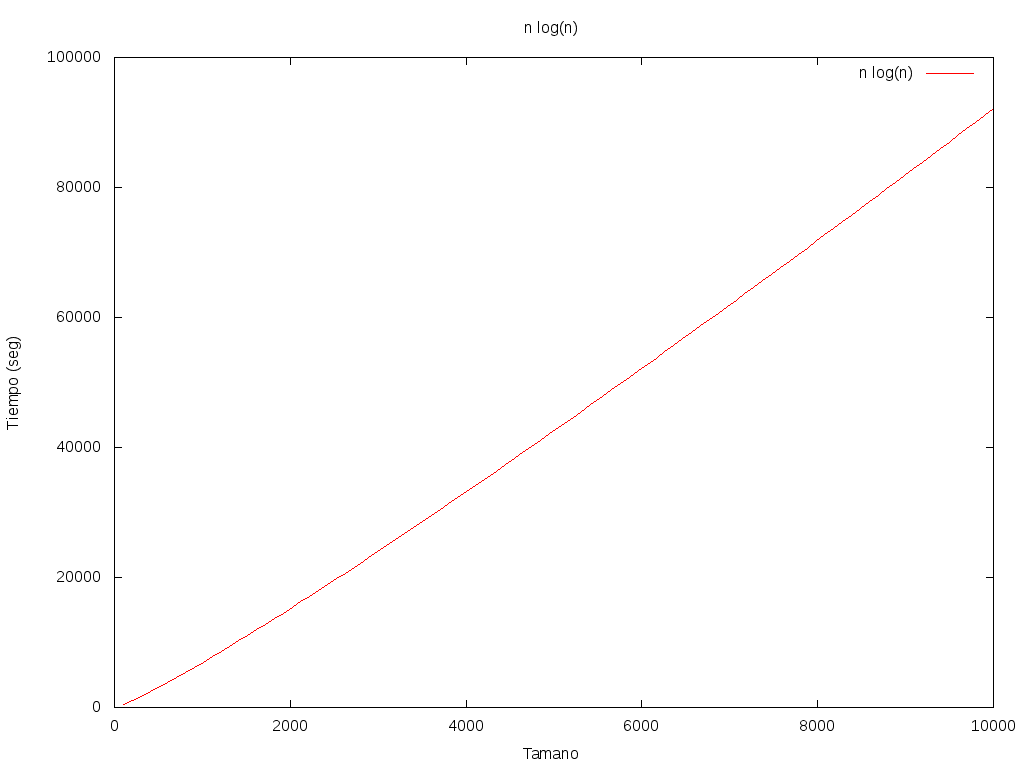
\includegraphics[width=0.5\linewidth]{imagenes/nlog(n)3.png}
		\caption{}
		\label{fig:E1}
	\end{figure}
	
\end{frame}
\subsection{Quick Sort}
\begin{frame}
	\frametitle{Quick Sort}
	La gráfica empírica obtenida ha sido:
	\begin{figure}
		\centering
		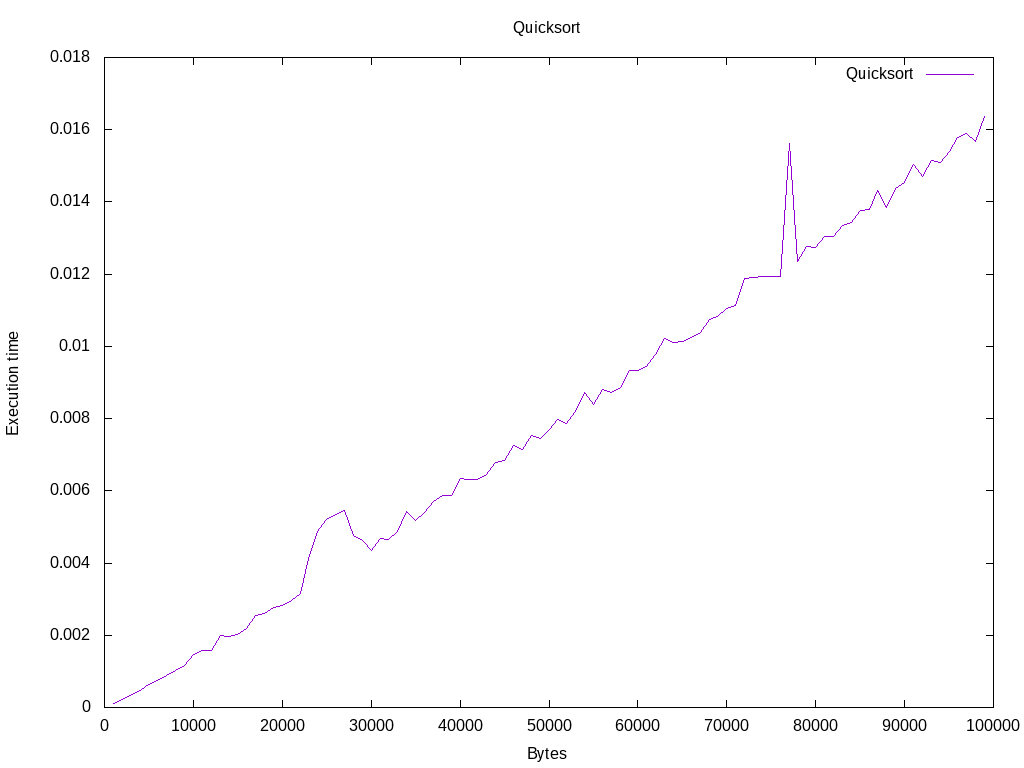
\includegraphics[width=0.7\linewidth]{imagenes/quicksort.png}
		\caption{}
		\label{fig:E4}
	\end{figure}
	
\end{frame}

\begin{frame}
	\frametitle{Quick Sort}
	La gráfica híbrida obtenida ha sido:
	\begin{figure}
		\centering
		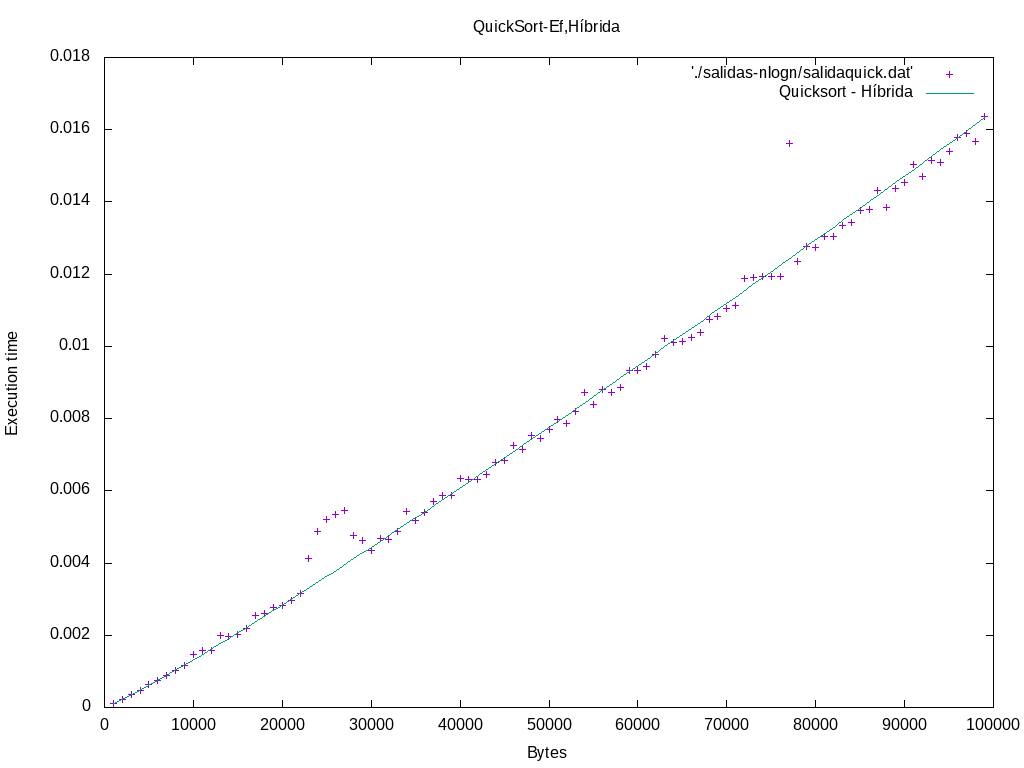
\includegraphics[width=0.7\linewidth]{imagenes/quicksort-hibrida.png}
		\caption{}
		\label{fig:E5}
	\end{figure}
\end{frame}
\subsection{Heap Sort}
\begin{frame}
	\frametitle{Heap Sort}
	La gráfica empírica obtenida ha sido:
	\begin{figure}
		\centering
		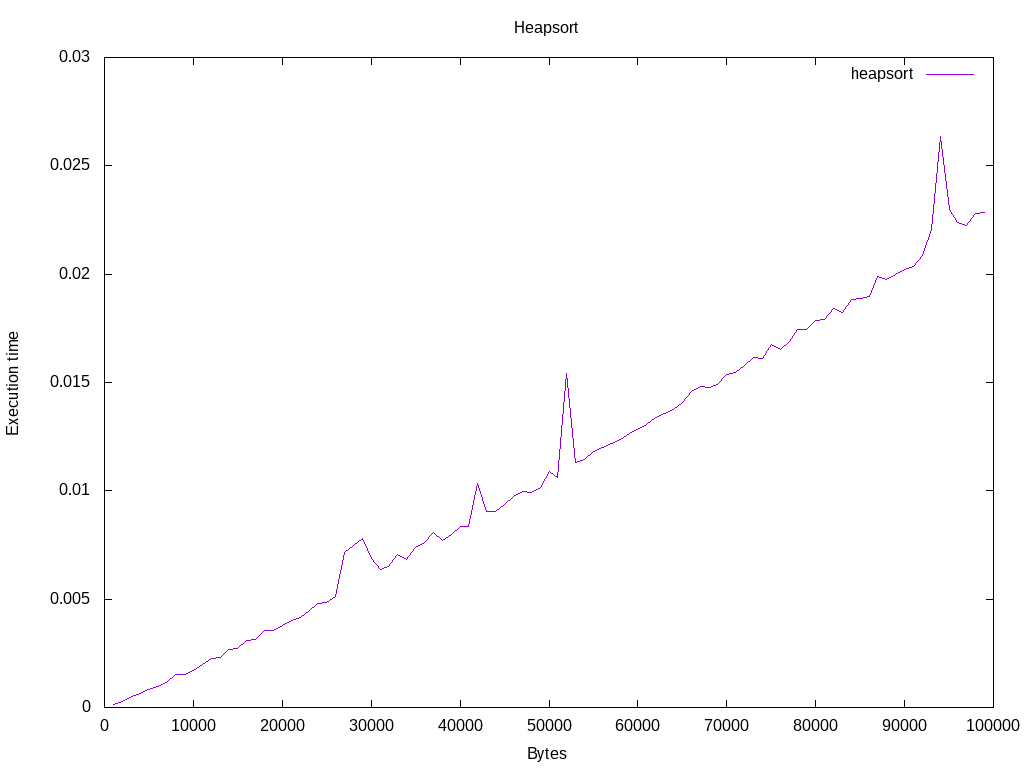
\includegraphics[width=0.7\linewidth]{imagenes/heapsort.png}
		\caption{}
		\label{fig:E4}
	\end{figure}
	
\end{frame}

\begin{frame}
	\frametitle{Heap Sort}
	La gráfica híbrida obtenida ha sido:
	\begin{figure}
		\centering
		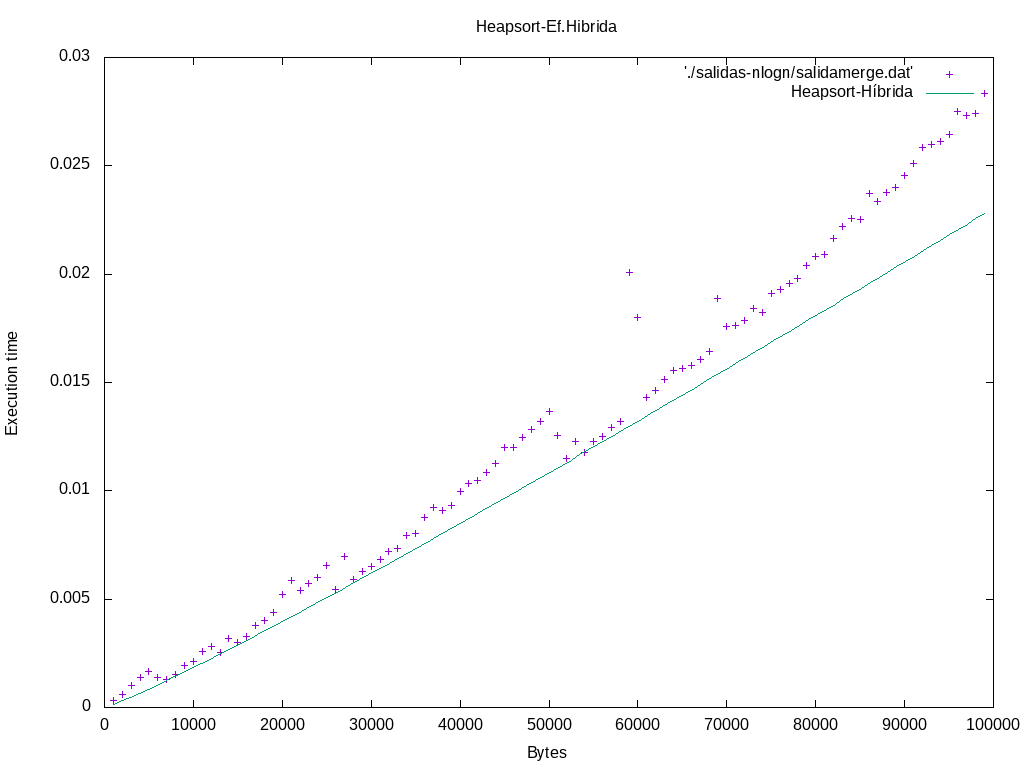
\includegraphics[width=0.7\linewidth]{imagenes/heapsort-hibrida.png}
		\caption{}
		\label{fig:E5}
	\end{figure}
\end{frame}
\subsection{Merge Sort}
\begin{frame}
	\frametitle{Merge Sort}
	La gráfica empírica obtenida ha sido:
	\begin{figure}
		\centering
		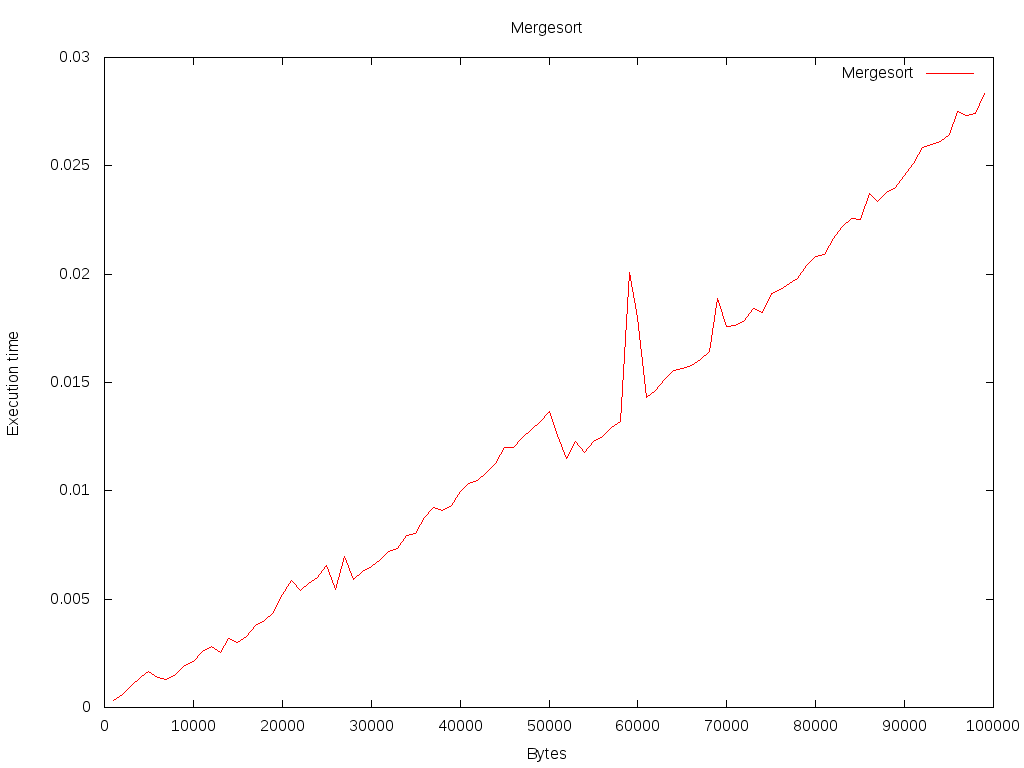
\includegraphics[width=0.7\linewidth]{imagenes/mergesort.png}
		\caption{}
		\label{fig:E4}
	\end{figure}
	
\end{frame}

\begin{frame}
	\frametitle{Merge Sort}
	La gráfica híbrida obtenida ha sido:
	\begin{figure}
		\centering
		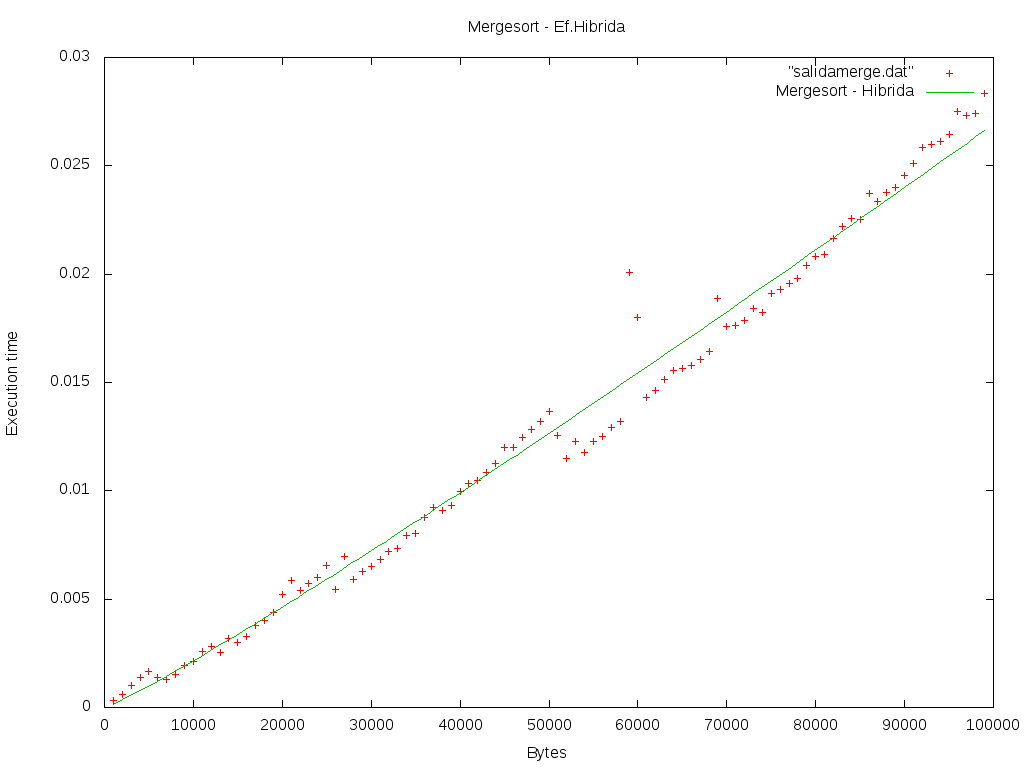
\includegraphics[width=0.7\linewidth]{imagenes/mergesort-hibrida.png}
		\caption{}
		\label{fig:E5}
	\end{figure}
\end{frame}
\section{Floyd}
\begin{frame}
	\frametitle{Floyd}
	La gráfica empírica obtenida ha sido:
	\begin{figure}
		\centering
		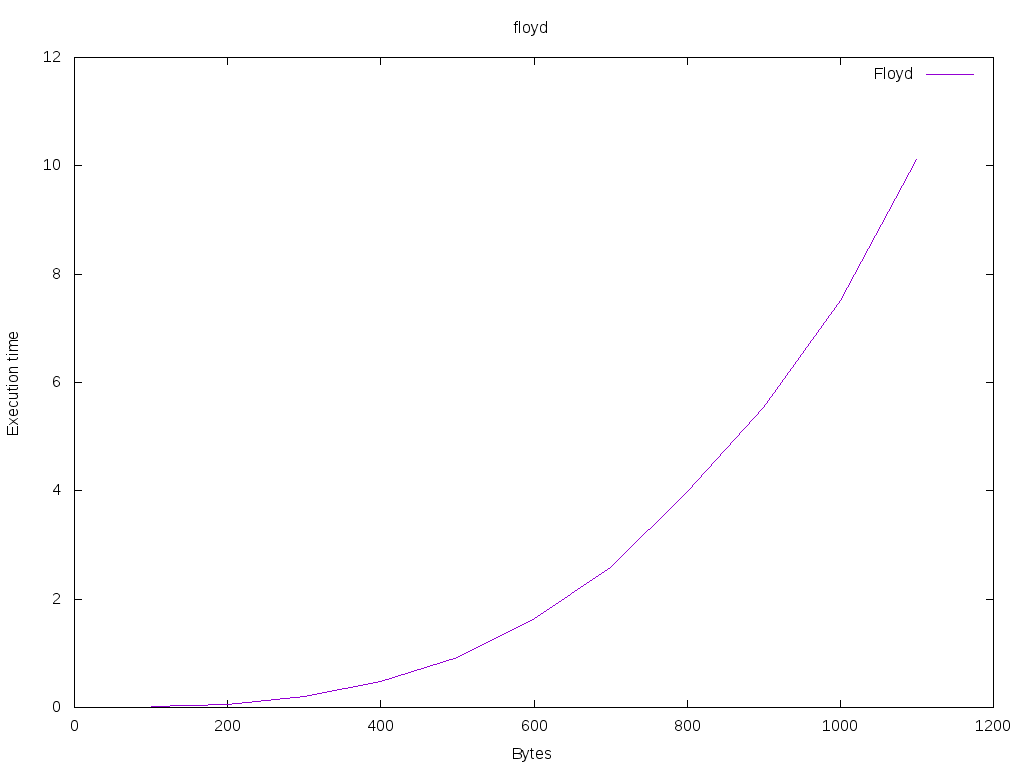
\includegraphics[width=0.7\linewidth]{imagenes/floyd.png}
		\caption{}
		\label{fig:E4}
	\end{figure}
	
\end{frame}

\begin{frame}
	\frametitle{Floyd}
	La gráfica híbrida obtenida ha sido:
	\begin{figure}
		\centering
		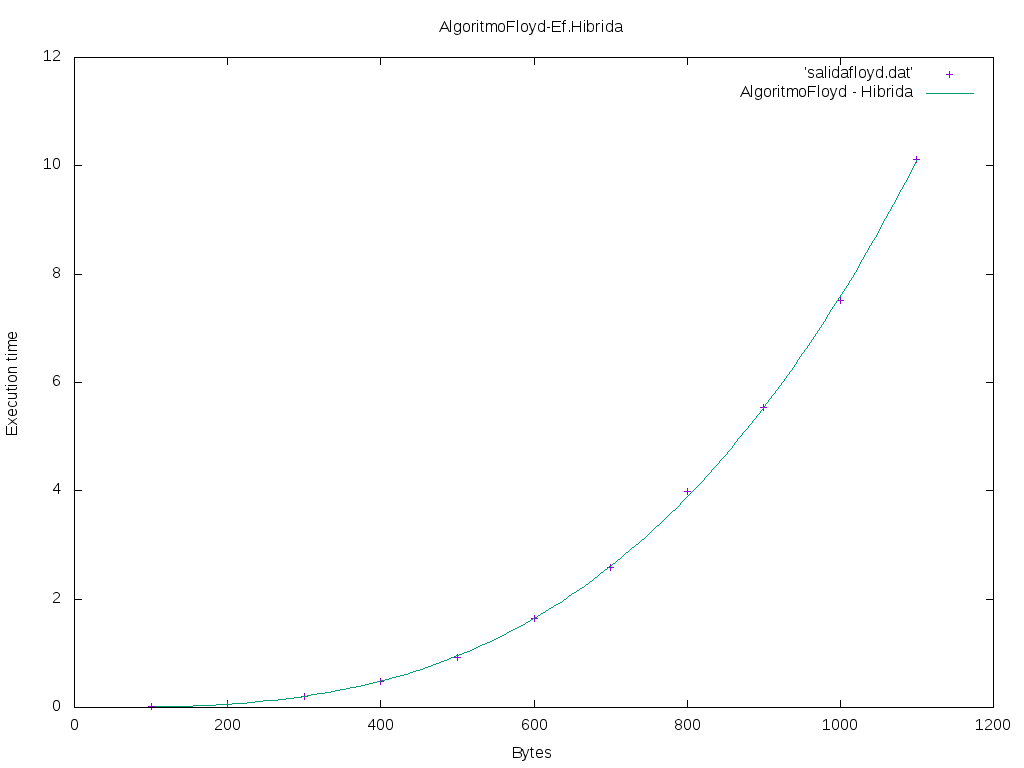
\includegraphics[width=0.7\linewidth]{imagenes/algoritmoFloyd-hibrida.png}
		\caption{}
		\label{fig:E5}
	\end{figure}
\end{frame}
\section{Hanoi}
\begin{frame}
	\frametitle{Hanoi}
	La gráfica empírica obtenida ha sido:
	\begin{figure}
		\centering
		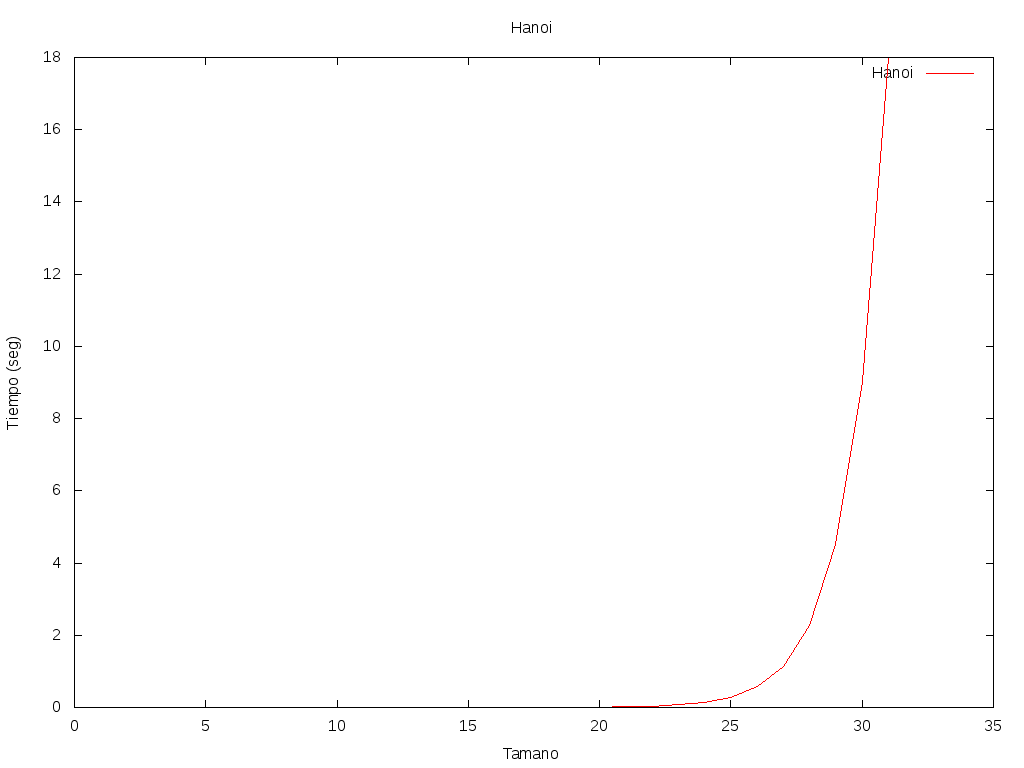
\includegraphics[width=0.7\linewidth]{imagenes/hanoiLines.png}
		\caption{}
		\label{fig:E4}
	\end{figure}
	
\end{frame}

\begin{frame}
	\frametitle{Hanoi}
	La gráfica híbrida obtenida ha sido:
	\begin{figure}
		\centering
		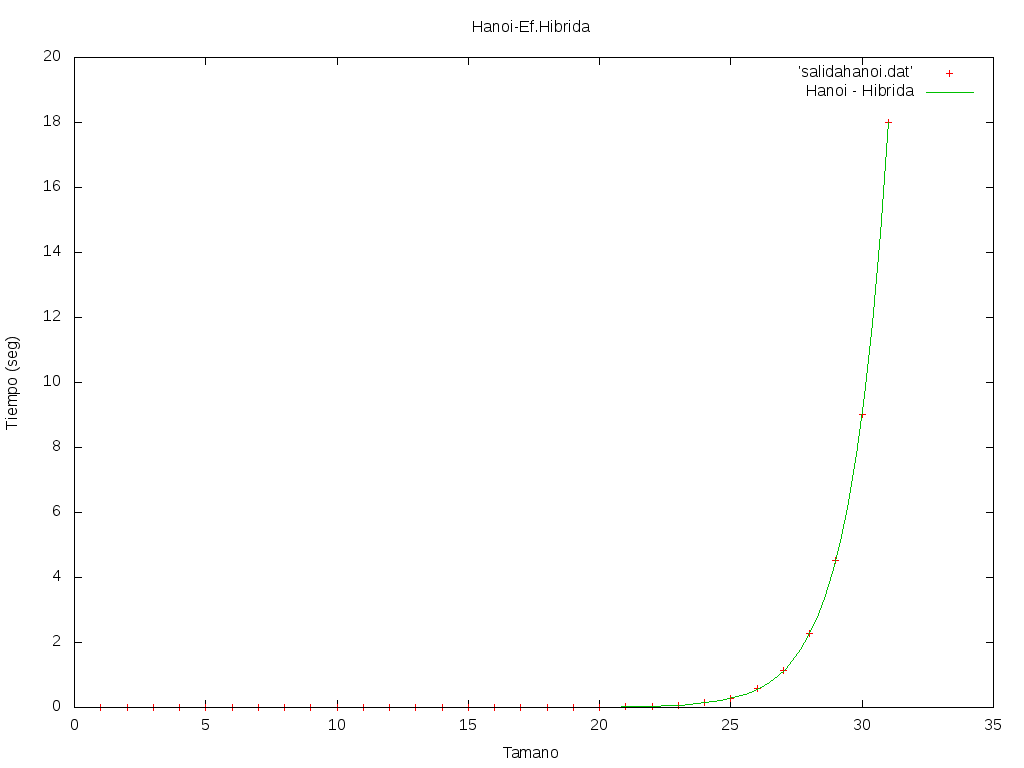
\includegraphics[width=0.7\linewidth]{imagenes/hanoi-hibrido.png}
		\caption{}
		\label{fig:E5}
	\end{figure}
\end{frame}



\begin{frame}
\Huge{\centerline{The End}}
\end{frame}

%----------------------------------------------------------------------------------------

\end{document} 